\documentclass[10pt]{exam}
\usepackage[hon]{template-for-exam}
\usepackage{endnotes,graphicx}
\usepackage{tikz,graphicx,enumitem,multicol,float,my-tikz-clipart,silence,cclicenses}
\graphicspath{{./figures/}}
\WarningFilter{latex}{Label `part}
\WarningFilter{latex}{There were multiply-defined labels}
\usetikzlibrary{arrows.meta}

\footer{}{\thepage}{\sc \myclass}


%\def\answer#1{\footnotetext{#1}}
%\def\myquestion{\item\stepcounter{footnote}}

\def\enoteheading{}
\def\answer#1{\endnotetext{#1}}
\def\theanswers{\theendnotes}
\def\myquestion{\item\stepcounter{endnote}}

\newenvironment{myquestions}{
  \begin{multicols}{2}\begin{enumerate}[resume]
}{
  \end{enumerate}\end{multicols}
}
\makeatletter
\patchcmd{\enit@setresumekeys}{\def}{\gdef}{}{}
\patchcmd{\enit@setresumekeys}{\def}{\gdef}{}{}
\makeatother

\newcommand{\myheading}[1]{\uplevel{\section*{#1}}
}
\newcommand{\mysubheading}[1]{\uplevel{\subsection*{#1}}
}

%uncomment if running Pandoc
% \renewcommand{\myheading}[1]{{\section*{#1}}}
% \renewcommand{\mysubheading}[1]{\subsection*{#1}}





\def\mytitle{Chapter 3 Homework B (Projectiles)}
\title{\mytitle}
\date{\today}

\def\mymaketitle{
  \begin{flushleft}
    {\LARGE \textbf \mytitle \par}
  \end{flushleft}
}

\newcommand{\bs}[2]{\textbf{#1} (\sc #2 Points)}


\newcommand{\GFig}[2]{  
  \begin{figure}[H]
    \centering
    \includegraphics[width=#2]{11_#1_Figure.jpg}
    \caption{Giancolli Figure 11-#1.}
    \label{11-#1}
  \end{figure}
}

\newcommand{\printeqs}{
  \section*{Equations} 
  
  \begin{center}
    \begin{tabular}{cccccc}
      $\bar{v} = \frac{\Delta x}{\Delta t}$       &   
      $\bar{a} = \frac{\Delta v}{\Delta t}$       &&
      $v = v_0 + a t$                             &
      $x = x_0 + v_0t + \frac{1}{2}at^2$          &
      $v^2 = v_0^2 + 2a \left( x - x_0 \right) $  \\
          & & & ``Old Faithful'' & ``Big Chalupa'' & ``Ain't Got No Time'' \\
    \end{tabular}

    %\vspace{1em}

    %$\SI{1}{\meter\per\second}=\SI{3.6}{\kilo\meter\per\hour}$
  \end{center}
}

\begin{document}
\maketitle
\begin{center}
  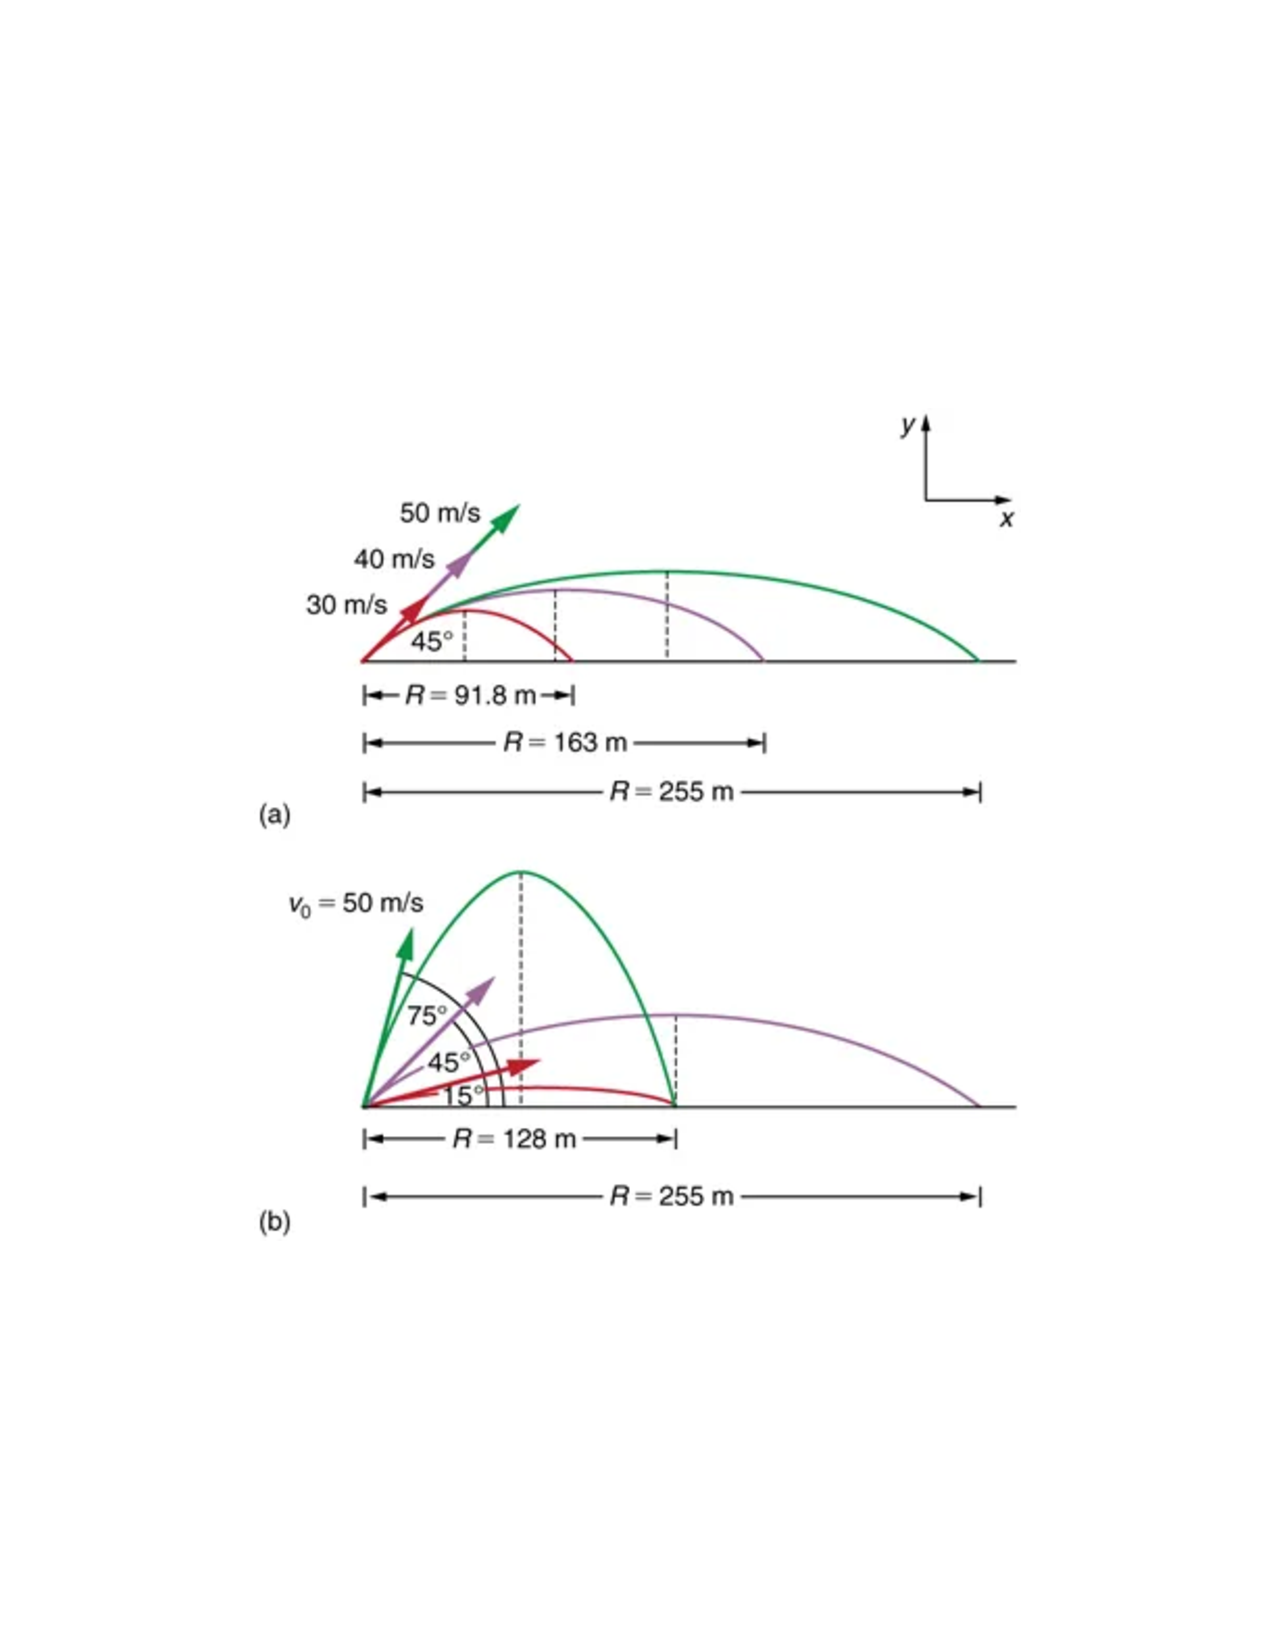
\includegraphics[height=3.2in]{3-38.pdf}
\end{center}




\vfill

\hrule
\vspace{0.2em}

\vspace{-.5em}

\begin{multicols}{3}
  \begin{center}

    $\vec{v} = \vec{v}_0 + \vec{a} t$
  
    \emph{\footnotesize ``Old Faithful''}
  
  
    $\vec{x} = \vec{x}_0 + \vec{v}_0 t + \frac{1}{2} \vec{a} t^2$
  
    \emph{\footnotesize``The Big Chalupa''}
  

    $\vec{v}^{\,2} = \vec{v}_0^{\,2}+ 2 \vec{a} \cdot 
    \left(\vec{x}-\vec{x}_0 \right)$

    \emph{\footnotesize ``Ain't Got No Time''}

  \end{center}
\end{multicols}

\vspace{-8pt}
\hrule
\vspace{1em}

\begin{minipage}{2.2in}
    \begin{center}
      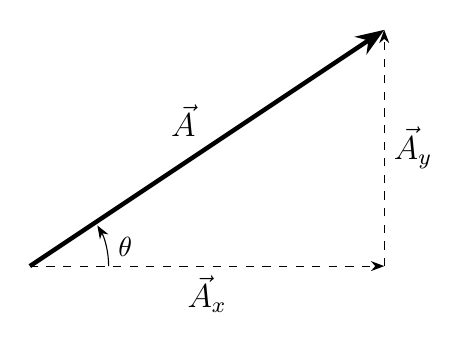
\begin{tikzpicture}[
        every node/.append style={},
        component/.append style={
          dashed,
          -{Stealth}
        },
        resultant/.append style={
          ultra thick,
          -{Stealth}
        },
    ]
      \draw[resultant] 
                (0,0) -- (4.5,3) 
                  node[midway,anchor=south east]{\large $\vec{A}$};
      \draw[component] 
                (0,0) 
                -- (4.5,0) 
                  node[midway,anchor=north]{\large $\vec{A}_x$} ;
      \draw[component] 
                (4.5,0)
                -- (4.5,3) 
                  node[midway,anchor=west]{\large $\vec{A}_y$} ;
      \draw[-Stealth] (1,0) node[anchor=south west]{$\theta$}
                arc[
                  start angle = 0,
                  end angle = 31, 
                  radius = 1
                ];
    \end{tikzpicture}


    \end{center}
  \end{minipage}
  %
  \begin{minipage}{4in}
    \begin{center}
      \begin{align*}
        A_x & = A \cos\theta &
        A_y & = A \sin\theta &
        \theta & = \tan^{-1} \left(\frac{A_y}{A_x}\right)
      \end{align*}

      \hrule 
      
      \begin{align*}
        R &= \frac{v_0^{\,2} \sin\left(2\theta\right)}{g}
      \end{align*}
      \vspace{0em}

      
    \end{center}
  \end{minipage}

  \vspace{1em}

    \hrule

  \begin{align*}
    \vec{v}_{AC} &= \vec{v}_{AB} + \vec{v}_{BC} &
    \vec{v}_{AB} &= -\vec{v}_{BA}
  \end{align*}

  \hrule

\section*{Selected Answers}

  \renewcommand{\enotesize}{\normalsize}
  \renewcommand{\enoteformat}{%
    \leftskip=1.8em
    \makebox[0pt][r]{\theenmark. }%
  }

  \hfill

  \begin{multicols}{2}
    \theanswers
  \end{multicols}


\vspace{1em}

\pagebreak

\hfill 

\pagebreak

\noindent
\textit{Questions and figures are from OpenStax} College Physics \textit{2nd ed (Chapter 3) or Giancolli} Physics: Principles with Applications \textit{7th ed. (Chapter 3) unless otherwise noted.}


\section*{Projectile Motion (Part II)}

Your work for these problems should include diagrams and knowns/unknowns.

\begin{myquestions}

\myquestion (Giancolli P26) \answer{12.5 s; 50 m}
Extreme-sports enthusiasts have been known to jump off the top of El Capitan, a sheer granite cliff of height 910~m in Yosemite National Park. Assume a jumper runs horizontally of the top of El Capitan with speed 4.0~m/s and enjoys a free fall until she is 150~m above the valley floor, at which time she opens her parachute (Figure~\ref{3-37}). (a) How long is the jumper in free fall? Ignore air resis- tance. (b) It is important to be as far away from the cliff
as possible before opening the parachute. How far from the cliff is this jumper when she opens her chute?

  \begin{figure}[H]
    \centering
    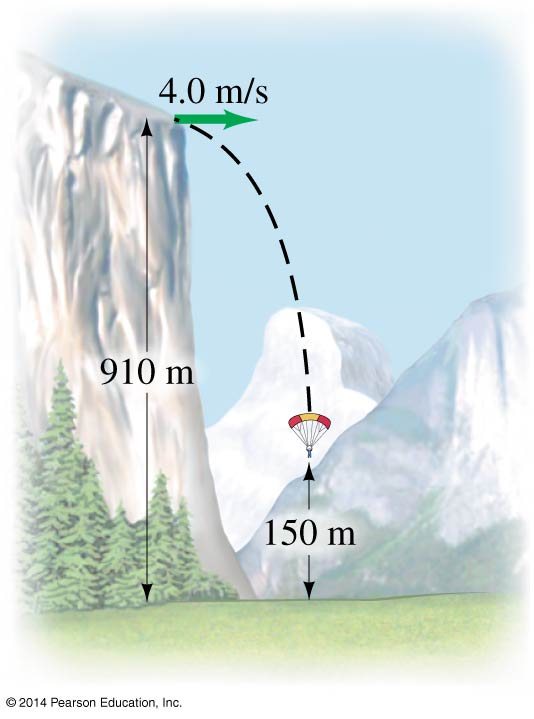
\includegraphics[width=1.5in]{G3-37.jpg}
    \caption{Fig 3-37 from Giancolli}
    \label{3-37}
  \end{figure}

\myquestion (OpenStax P28) \answer{(a) 7 busses; (b) margin of error is about 6.7~m}
(a) A daredevil is attempting to jump his motorcycle over a line of buses parked end to end by driving up a $32^\circ$  ramp at a speed of 40.0~m/s. How many buses can he clear if the top of the takeoff ramp is at the same height as the bus tops and the buses are 20.0~m long? (b) Discuss what your answer implies about the margin of error in this act---that is, consider how much greater the range is than the horizontal distance he must travel to miss the end of the last bus. (Neglect air resistance.)

\myquestion (OpenStax P33)
The cannon on a battleship can fire a shell a maximum distance of 32.0~km. (a) Calculate the initial velocity of the shell. (b) What maximum height does it reach? (At its highest, the shell is above 60\% of the atmosphere—but air resistance is not really negligible as assumed to make this problem easier.) \answer{(a) 560 m/s; (b) 8000 m} 




\end{myquestions}

\pagebreak

\begin{myquestions}



\myquestion (OpenStax P29) \answer{(a) $18.4^\circ$; (b) max height is 6.23~m, so it makes it over the branch}
An archer shoots an arrow at a 75.0~m distant target; the bull's-eye of the target is at same height as the release height of the arrow. (a) At what angle must the arrow be released to hit the bull's-eye if its initial speed is 35.0~m/s? %In this part of the problem, explicitly show how you follow the steps involved in solving projectile motion problems. 
(b) There is a large tree halfway between the archer and the target with an overhanging horizontal branch 3.50~m above the release height of the arrow. Will the arrow go over or under the branch?




% \myquestion (OpenStax P34)
% An arrow is shot from a height of 1.5 m toward a cliff of height $H$. It is shot with a velocity of 30~m/s at an angle of $60^\circ$ above the horizontal. It lands on the top edge of the cliff 4.0~s later. (a) What is the height of the cliff? (b) What is the maximum height reached by the arrow along its trajectory? (c) What is the arrow's impact speed just before hitting the cliff?
% \answer{(a) 27.0 m; (b) 13.2 m/s (c) 20 m/s}

% \myquestion (OpenStax P41)
% An owl is carrying a mouse to the chicks in its nest. Its position at that time is 4.00 m west and 12.0 m above the center of the 30.0 cm diameter nest. The owl is flying east at 3.50 m/s at an angle 30.0º below the horizontal when it accidentally drops the mouse. Is the owl lucky enough to have the mouse hit the nest? To answer this question, calculate the horizontal position of the mouse when it has fallen 12.0 m. \answer{4.23 m forward of drop location; misses the nest}

% \myquestion (OpenStax P45) 
% In 2007, Michael Carter (U.S.) set a world record in the shot put with a throw of 24.77~m. What was the initial speed of the shot if he released it at a height of 2.10~m and threw it at an angle of $38.0^\circ$ above the horizontal? (Although the maximum distance for a projectile on level ground is achieved at $45^\circ$  when air resistance is neglected, the actual angle to achieve maximum range is smaller; thus, $38^\circ$  will give a longer range than $45^\circ$ in the shot put.) \answer{15.0 m/s}


\myquestion (Giancolli P29) \answer{22.3 m}
A shot-putter throws the ``shot'' (mass 73~kg) with an initial speed of 14.4~m/s at a $34.0^\circ$ angle to the horizontal.  Calculate the horizontal distance traveled by the shot if it leaves the athlete's hand at a height of 2.10~m above the ground.


\myquestion (Giancolli P56) \answer{6.65 m/s}
Romeo is throwing pebbles gently up ot Juliet's window, and he wants the pebbles to hit the window with only a horizontal component of velocity. He is standing at the edge of a rose garden 8.0~m below her window and 8.5~m from the base of the wall (Figure~\ref{3-49}). How fast are the pebbles going when they hit her window?

  \begin{figure}[H]
    \centering
    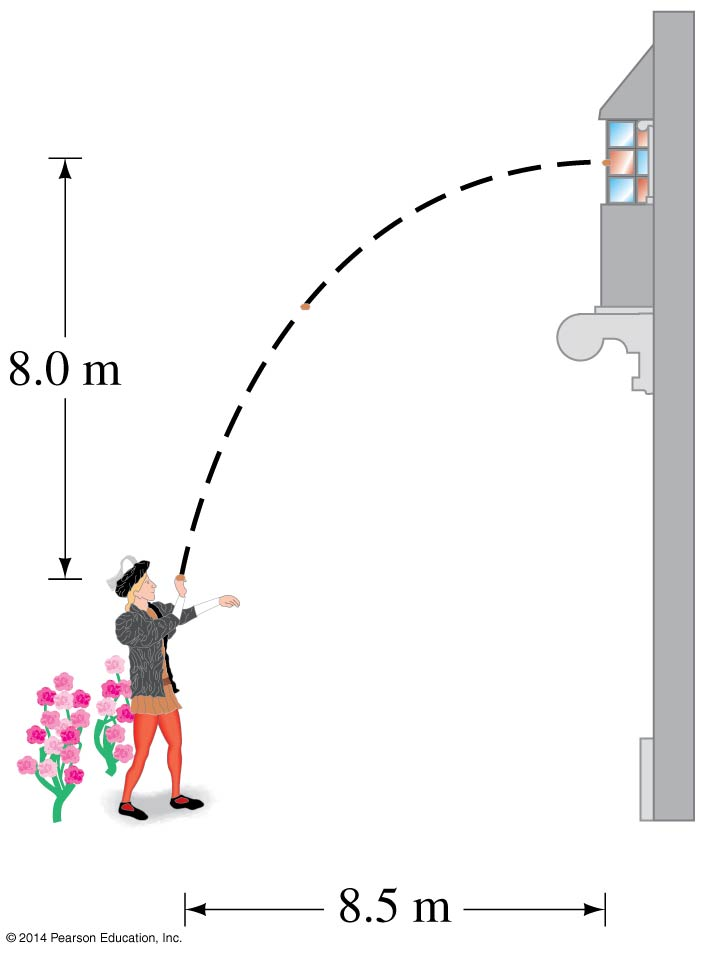
\includegraphics[width=1.5in]{G3-49.jpg}
    \caption{Fig 3-49 from Giancolli}
    \label{3-49}
  \end{figure}

\hfill [See \#\ref{proj-i}-\#\ref{proj-f} for additional practice]

\end{myquestions}


\pagebreak

\section*{Projectile Conceptual Questions}

Please answer each question in at least one complete sentence

\begin{enumerate}[resume]

  \myquestion (Original question) A projectile is launched at an angle $25^\circ$ above horizontal.  When (if ever) is its velocity zero? \vs
  \myquestion (OpenStax CQ15) For a fixed initial speed, the range of a projectile is determined by the angle at which it is fired. For all but the maximum, there are two angles that give the same range. Considering factors that affect the ability of an archer to hit a target, such as wind, explain why the smaller angle (closer to the horizontal) is preferable. On the other hand, why does the punter in a football game use the higher trajectory? \vs
  \myquestion (Giancolli CQ15) A projectile is launched at an upward angle of $30^\circ$ to the horizontal with a speed of 30~m/s.  How does the horizontal component of its velocity 1.0~s after launch compare with its horizontal component of velocity 2.0~s after launch, ignoring air resistance?  Explain. \vs



\end{enumerate}

\pagebreak

\section*{Relative Motion}

\begin{myquestions}



\myquestion (Original Problem) \answer{2.70 m/s east; 0.30 m/s east}
A moving walkway travels east at 1.50 m/s. A student walks east on it at 1.20 m/s relative to the walkway, then turns and walks west at the same speed relative to the walkway. Find the student's velocity relative to the ground in each case.


\myquestion (Giancolli P38) 
A jogger is exercising on the deck of a cruise ship. The ship moves forward at a constant speed of 8.5 m/s relative to the water.
\begin{parts}
  \part While running toward the bow (front) of the ship, the jogger's speed relative to the ship is 2.0 m/s. Determine the jogger's velocity relative to the water.
  \part Later, the jogger runs toward the stern (rear) of the ship at the same speed relative to the ship. What is the jogger's velocity relative to the water in this case?
\end{parts}
\answer{(a) 10.5 m/s; (b) 6.5 m/s}

\myquestion (Giancolli P39) \answer{1.66 m/s @ 65.0$^\circ$ E of N}
Huck Finn stands on a raft drifting down the Mississippi River. The raft moves at 1.50 m/s relative to the riverbank. Huck walks at 0.70 m/s relative to the raft, moving perpendicular to the raft's motion (that is, across the raft). Determine Huck's velocity (both magnitude and direction) relative to the riverbank.

  \begin{figure}[H]
    \centering
    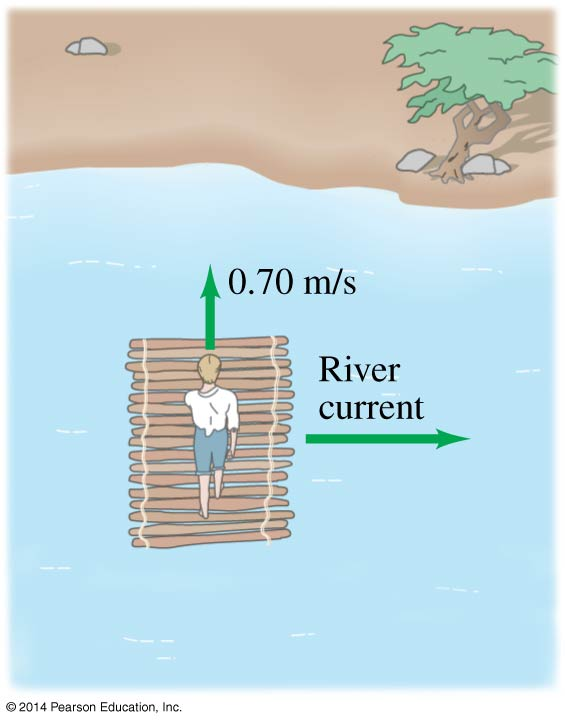
\includegraphics[width=1.5in]{G3-42.jpg}
    \caption{Fig 3-42 from Giancolli. Relative velocity of Huck walking across a drifting raft.}
    \label{3-42}
  \end{figure}


\myquestion (OpenStax P57) \answer{8.05~m/s @ $81.8^\circ$ N of E}
A ship sets sail from Rotterdam, The Netherlands, heading due north at 7.00 m/s relative to the water. The local ocean current is 1.50 m/s in a direction $40.0^\circ$  north of east. What is the velocity of the ship relative to the Earth?


\hfill [See \#\ref{rel-i}-\#\ref{rel-f} for additional practice]

\end{myquestions}

\pagebreak

\section*{Relative Velocity Conceptual Questions}

\begin{enumerate}[resume]
  \myquestion (OpenStax CQ19) If someone is riding in the back of a pickup truck and throws a softball straight backward, is it possible for the ball to fall straight down as viewed by a person standing at the side of the road? Under what condition would this occur? How would the motion of the ball appear to the person who threw it? \vs
  \myquestion (OpenStax CQ20) The hat of a jogger running at constant velocity falls off the back of his head. Draw a sketch showing the path of the hat in the jogger's frame of reference. Draw its path as viewed by a stationary observer. \vs
  \myquestion (Giancolli CQ19) If you are riding on a train that speeds past another train moving in teh same direction on an adjacent track, it appers that the other train is moving backward.  Why? \vs
\end{enumerate}

\pagebreak



\section*{Additional Practice}
These problems are provided for extra practice.  They are \emph{not required} and there is no bonus for doing them.
  
\begin{myquestions}
  
\myquestion (Giancolli P20) \answer{7.7 m/s} \label{proj-i}
A ball is thrown horizontally from the roof of a building 7.5~m tall and lands 9.5~m from the base. What was the ball's initial speed?


\myquestion (OpenStax P40)
An eagle is flying horizontally at a speed of 3.00~m/s when the fish in her talons wiggles loose and falls into the lake 5.00~m below. Calculate the velocity of the fish relative to the water when it hits the water. \answer{10.3~m/s @ 73.1$^\circ$ below horiz}

\myquestion (OpenStax P43) \label{proj-f}
Can a goalkeeper at her/his goal kick a soccer ball into the opponent's goal without the ball touching the ground? The distance will be about 95 m. A goalkeeper can give the ball a speed of 30 m/s. \answer{No. Max range $\approx 92$ m}


% \myquestion (Giancolli P46) \answer{}
% A swimmer is capable of swimming 0.60~m/s in still water. (a) If she aims her body directly across a 45-m-wide river whose current is 0.50~m/s, how far downstream (from a point opposite her starting point) will she land? (b) How long wil it take her to reach the other side?

\myquestion (Original Problem) \answer{2.16 m/s at 33.7$^\circ$ east of north} \label{rel-i}
A swimmer can swim 1.80 m/s north relative to the water. A river current flows 1.20 m/s east. Find the swimmer's velocity relative to the shore.

\myquestion (Original Problem) \answer{228 km/h at 15.3$^\circ$ west of north}
A plane has an air speed of 220 km/h due north. The wind blows 60.0 km/h due west. Find the plane's ground speed and direction.

\myquestion (Giancolli P41, modified) \label{rel-f}
 Two planes approach each other head on.  Each has a speed of 200 m/s, and they spot each other when they are initially 10 km apart.  How much time to the airplanes have to take evasive action?
 \answer{25 s}

\end{myquestions}

\hrule

\section*{Bonus}

You will be given bonus if you complete these problems \emph{on a separate sheet of paper}
  
\begin{myquestions}


\myquestion (OpenStax P35)
In the standing broad jump, one squats and then pushes off with the legs to see how far one can jump. Suppose the extension of the legs from the crouch position is 0.600 m and the acceleration achieved from this position is 1.25 times the acceleration due to gravity, $g$. How far can they jump? State your assumptions. (Increased range can be achieved by swinging the arms in the direction of the jump.) \answer{1.50 m}

\myquestion (OpenStax P47)
A football player punts the ball at a $45.0^\circ$ angle. Without an effect from the wind, the ball would travel 60.0~m horizontally. (a) What is the initial speed of the ball? (b) When the ball is near its maximum height it experiences a brief gust of wind that reduces its horizontal velocity by 1.50 m/s. What distance does the ball travel horizontally?


\myquestion (Giancolli P42)
A boat moves across a still lake at 1.70 m/s. A passenger walks up a flight of stairs on the boat at a speed of 0.60 m/s relative to the boat. The stairs are oriented at a $45^\circ$ angle in the forward direction, as shown in Figure~\ref{3-43}.  Determine the velocity of the passenger relative to the water.
\answer{8.05 m/s @ 81.8$^\circ$ N of E}

  \begin{figure}[H]
    \centering
    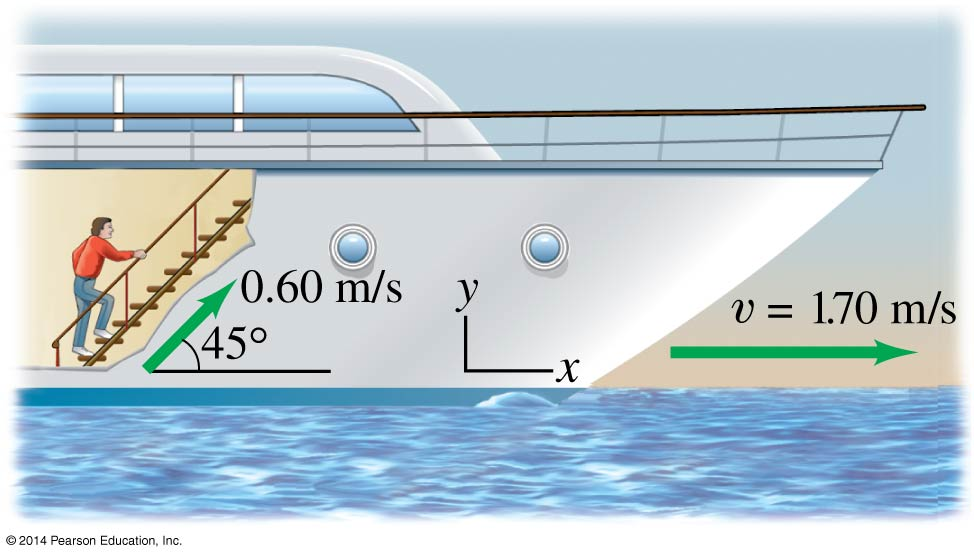
\includegraphics[width=2.5in]{G3-43.jpg}
    \caption{Fig 3-43 from Giancolli}
    \label{3-43}
  \end{figure}

\myquestion (Giancolli P50)
An airplane has an airspeed of 580 km/h and must fly along a straight path directed $38^\circ$ north of east. A steady wind of 82~km/h blows from the north.  In what direction should the airplane head in order to maintain the required path?


% \myquestion (OpenStax P61)
% A sandal is dropped from the top of a 15.0-m-high mast on a ship moving at 1.75~m/s due south. Calculate the velocity of the sandal when it hits the deck of the ship: (a) relative to the ship and (b) relative to a stationary observer on shore. (c) Discuss how the answers give a consistent result for the position at which the sandal hits the deck.

% \myquestion (OpenStax P67)
% An ice hockey player is moving at 8.00~m/s when they hit the puck toward the goal. The speed of the puck relative to the player is 29.0~m/s. The line between the center of the goal and the player makes a $90^\circ$ angle relative to their path as shown in Figure~\ref{3-60}. What angle must the puck's velocity make relative to the player (in their frame of reference) to hit the center of the goal?

%   \begin{figure}[H]
%     \centering
%     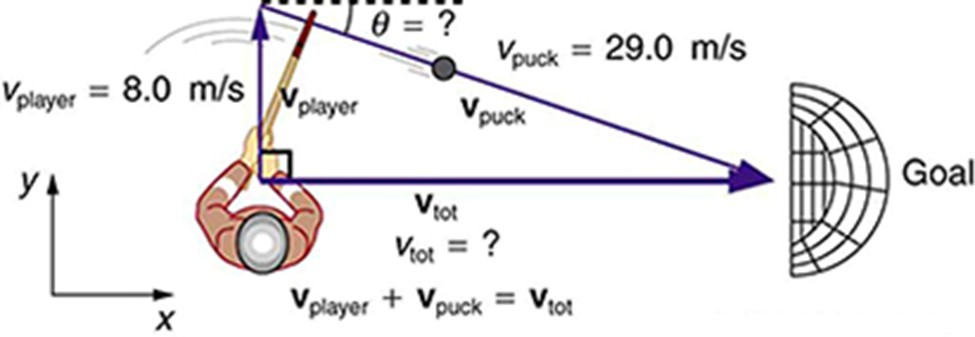
\includegraphics[width=3.1in]{3-60.jpg}
%     \caption{(OpenStax Fig 3.60) An ice hockey player moving across the rink must shoot backward to give the puck a velocity toward the goal.}
%     \label{3-60}
%   \end{figure}


  
\end{myquestions}



\end{document}